\chapter[Algoritmos]{Flujos de trabajo sobre cómputo en la nube}
\label{chap:algorithm}

En este capítulo, describiremos el algoritmo que es la pieza clave del sistema para agendar tareas de un flujo de trabajo en infraestructura de cómputo en la nube, tomando en cuenta los lineamientos de diseño propuestos anteriormente.



\section{Antecedentes}

Un área de investigación activa es la planificación de tareas a nivel de procesador (CPU's), en donde se asume que se tiene un procesador cuyos núcleos son idénticos e intercambiables. En los trabajos de investigación referentes a esta área se consideran a los grafos dirigidos acíclicos como los modelos de tareas más generales. Así, en el trabajo de Saifullah et al. \cite{saifullah2013multi}, se transforma un grafo dirigido acíclico en un conjunto de tareas secuenciales con secciones que se ejecutan en paralelo.


% Podemos hacer esto aún más abstracto y combinarlo con la teoría de Pinedo

% EFT: Earliest-Finish Time
% DM: Deadline Monotonic
% EDF: Earliest-Deadline First
% Global EDF
% Partitioned EDF

% how to enable theory with processor teory
% I think my thesis is that weird link, with the basic paper
% no hay que olvidar que hay que optimizar tiempo, dinero

% ya sabemos que es NP-hard, asi que nos enfocaremos en el problema

% Primero, tienes recursos 'infinitos', solo sujetos a presupuesto
% puedes averiguar el numero maximo de maquinas a levantar con el modelo de tareas paralelar
% simplemente cuentas el segmento con el mayor numero de paralelizaciones

Es muy común que los servicios de cómputo en la nube se pague la utilización de las máquinas virtuales por hora, dejando sin cobrar porciones de hora no utlizadas. Además, se pueden solicitar tantos recursos como se requieran, limitándose solamente al presupuesto disponible. Tambi\'en, estas máquinas virtuales son recursos variados; pueden ser desde máquinas con un solo procesador, hasta m\'aquinas virtuales con grandes cantidades de memoria y m\'ultiples procesadores.

De acuerdo al primer cap\'itulo del libro de Pinedo \cite{pinedo2012scheduling} hay esfuerzos para clasificar los problemas de planificación en general. Sin embargo, la clasificación presentada en este trabajo sólo contempla los problemas que optimizan una sola métrica, aunque, se puede utilizar una combinación de funciones objetivo a optimizar. Sin embargo, esta forma de atacar el problema de planificación multiobjetivo no garantiza evaluar todas las posibles opciones. 

% Hacer puente entre las teorías de Buyya y Jia Yu y las teorías de Pinedo

% Hay que leer los papers de arquitectura

\section{Ejecución de flujos de trabajo}

Si bien en la literatura hay múltiples algoritmos de planificación publicados por la comunidad científica, éste es sólo una parte (muy importante) de un sistema administrador de flujos de trabajo. En el caso de este trabajo, dividimos todo el proceso en cuatro fases:

\begin{enumerate}
\item{Planificación}
\item{Ejecución}
\item{Descarga de resultados}
\end{enumerate}



\subsection{Planificación: el algoritmo Ciego}

La idea base del algoritmo es lidiar con las dependencias, ya que éstas generan restricciones sobre el problema. Otra característica a aprovechar es el hecho de que los recursos de cómputo en la nube pueden ser tratados como \emph{efímeros}, es decir, pueden ser creados y destruidos conforme se requiera.

De esta forma, el primer paso del algoritmo de planificación es dividir el flujo de trabajo en segmentos consecutivos, con la propiedad de que un segmento sólo dependa de la ejecución completa del segmento anterior.

\subsubsection{Segmentación del flujo de trabajo}

Para generar los segmentos, se utiliza la definición de Saifullah et. al \cite{saifullah2013multi} basada en la profundidad de cada nodo del grafo dirigido acíclico que representa el flujo de trabajo.

\begin{defn}

La \textbf{profundidad} $H$ de una tarea $t$ de un flujo de trabajo está definida como:

\begin{displaymath}
H(x) = \left\{
     \begin{array}{lr}
       \max_{u \in \text{Padres}(t) } H(u) + 1 & : \text{Padres}(t) \neq \varnothing \\
       1                                       & : \text{Padres}(t) = \varnothing
     \end{array}
   \right.
\end{displaymath}

\noindent Donde $\text{Padres}(t)$ es el conjunto de tareas que inmediatamente preceden a la tarea $t$, es decir, aquellas tareas $u$ que tienen una dependencia de orden que va a la tarea $t$.
\end{defn}

La profundidad $H$ es definida recursivamente sobre las depdendencias que tiene cada tarea en un flujo de trabajo. Las tareas que no tienen dependencias (o padres), tendrán profundidad $H = 1$; mientras que las tareas que tengan dependencias, tendrán profundidad igual a la profundidad más alta de alguna de sus dependencias sumada en 1. Este último sumando representa, por definición, la profundidad que tiene cada una de las tareas del flujo de trabajo sin importar sus dependencias. Por lo tanto, las tareas siempre tendrán profundidades $H$ diferentes a las profunidades $H'$ de sus padres (o dependencias). Así, se puede definir los segmentos de un flujo de trabajo de la siguiente forma:

\begin{defn}
Un \textbf{segmento} $S_h$ de un flujo de trabajo es un conjunto de tareas que tienen la misma \emph{profundidad} $h$, es decir: 

\begin{displaymath}
S_h = \{ t \in T \mid H(t) = h \}
\end{displaymath}

\end{defn}

En la figura \ref{fig:DAG_to_segment} se puede apreciar un ejemplo de la segmentación, en donde se puede ver que a cada tarea del flujo de trabajo se le asigna un segmento. Si ejecutarámos las tareas de ordenadas en segmentos ordenados por su profunidad $h$, podríamos asegurar que sólo es necesario verificar que las tareas del segmento $h - 1$ estén completas para ejecutar las tareas del segmento $h$; esto asegura que se respeten las restricciones de orden del flujo de trabajo.

\begin{figure}
\begin{center}
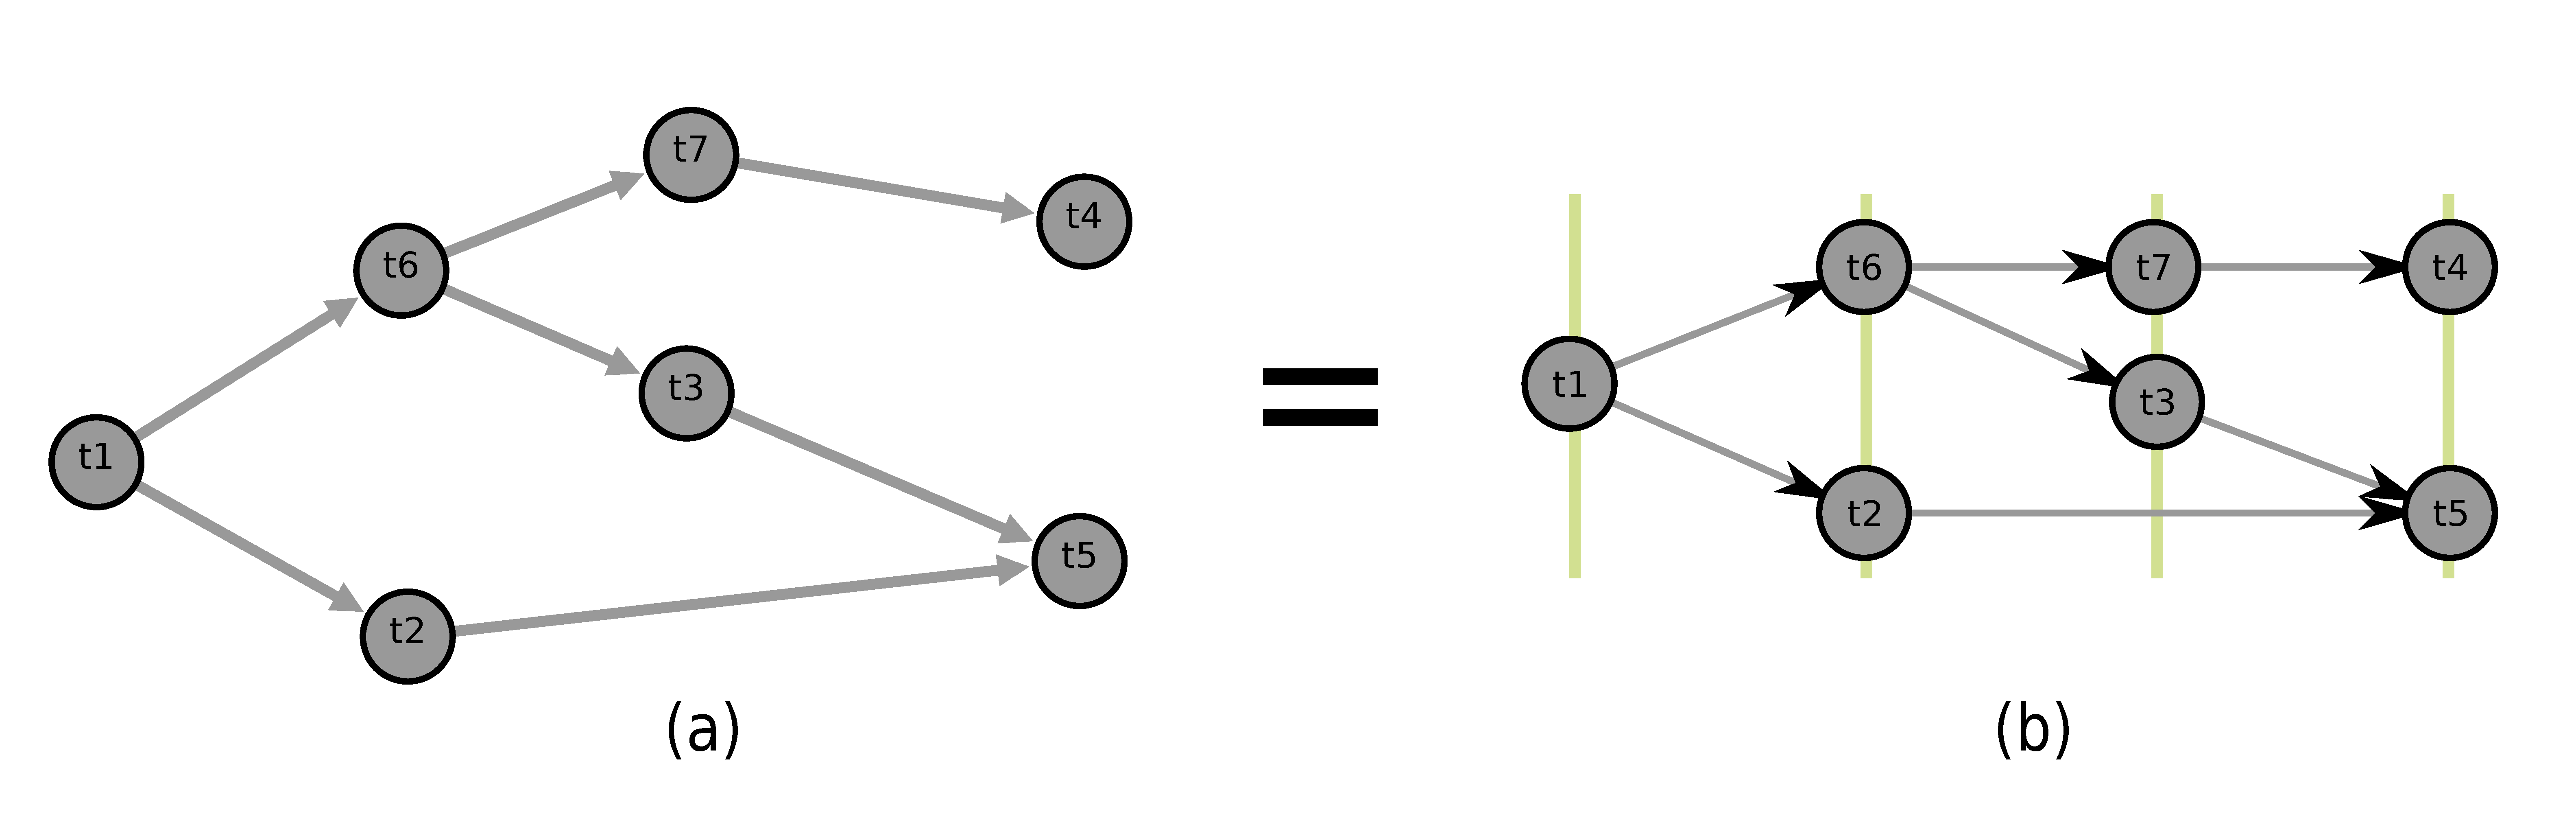
\includegraphics[width=1.0\textwidth]{imagenes/DAG_to_segment.pdf}
\end{center}
\caption{Transformación de un flujo de trabajo (a) a segmentos (b)}
\label{fig:DAG_to_segment}
\end{figure}

Otro punto a notar es que hay un límite en el número de tareas concurrentes que es posible ejecutar debido a las restricciones. Esto implica que a lo sumo hay un número finito de recursos concurrentes que se necesitan para correr el flujo de trabajo. Este límite equivale al máximo de tareas de los segmentos que conforman el flujo de trabajo.

En el pseudocódigo \ref{alg_blind_segments}, se calculan los segmentos de un flujo de trabajo.

\begin{algorithm}
\caption{Segmentación de un flujo de trabajo}
\label{alg_blind_segments}
\begin{algorithmic}[1]
\Require{Un flujo de trabajo $workflow$}
\Ensure{Un mapa con los segmentos de cada tarea del flujo de trabajo}
\Procedure{get\_task\_segments}{$workflow$}
	\State $visited \gets$ Diccionario
	\State $segment \gets$ Diccionario
	\For{$t \in workflow.tasks$}
		\State \Call{get\_segment}{$t$}
	\EndFor
	\State \Return $segment$
\EndProcedure

\Procedure{get\_segment}{$task$}
	\State $visited[task] \gets True$
	\State $max\_seg \gets 0$
	\If{$ \lnot (task \in segment)$}
		\State $segment[task] \gets 0$
		\For{$p \in task.parents$}
			\State $v \gets \Call{get\_segment}{p}$
			\If{$v > max\_seg$}
				\State $max\_seg = v$
			\EndIf
		\EndFor
		\State $segment[task] \gets max\_seg + 1$
	\EndIf
	\State \Return $segment[task]$
\EndProcedure


%\Procedure{estimate\_resources}{$workflow$}
%	\State $segments \gets \Call{$get\_task\_segments$}$
%	\State $segmentsHeight \gets $ Diccionario
%	\State $max\_segment \gets 0$
%	\For{$k$, $v$ in $segments$}
%		\State $segment \gets v$
%		\If{$segment \in segmentsHeight$}
%			\State $val \gets segmentsHeight[ segment ]$
%		\Else
%			\State $val \gets 0$
%		\EndIf
%		\State $val \gets val + 1$
%		\State $max\_segment \gets \max(val, max\_segment)$
%	\EndFor
%\EndProcedure

\Procedure{toSegmentList}{$segments$}
	\State{$segmentList \gets Diccionario$}
	\For{$(t,s) \in segments$}
		\If{$s \in segmentList$}
			\State{$taskList \gets segmentList[s]$}
		\Else
			\State{$taskList \gets Conjunto vacio$}
			\State{$segmentList[s] \gets taskList$}
		\EndIf
		\State{Agregar $t$ a $taskList$}
	\EndFor
	\State{\Return{$segmentList$}}
\EndProcedure	
\end{algorithmic}
\end{algorithm}

\subsubsection{Asignación de configuraciones a tareas de un segmento}

Ahora, el cómputo en la nube abre otras posibilidades que no se pueden realizar en los entornos de cómputo distribuido tradicionales, como el hecho de poder solicitar máquinas virtuales de acuerdo a la demanda. De esta forma, con las tareas del flujo de trabajo segmentadas, se puede ver a cada segmento como un conjunto de tareas independientes. Así, se puede usar un algoritmo de programación dinámica que pueda encontrar la asignación óptima de máquinas virtuales y tareas entre cada segmento.

%Así, este algoritmo se puede ver como el algoritmo de la mochila \emph{inverso} con múltiples mochilas, en donde las mochilas son las posibles configuraciones y las tareas son objetos que deben ser \emph{embolsados}. 

Así, este algoritmo se puede ver como un algoritmo de búsqueda exhaustiva. El objetivo de este algoritmo es encontrar aquella asignación que pueda asignar todas las tareas maximizando el uso de los núcleos de las posibles configuraciones de la máquinas virtuales, sujeto a una condición de optimalidad. Para este caso, la condición de optimalidad es definida a trav\'es de una funci\'on de costo parcial, especificada por el usuario. 

Por el momento, para hacer la relaci\'on entre configuraciones y tareas, se asume que cada tarea ocupa un núcleo de una máquina virtual y que todas las posibles configuraciones de máquinas virtuales del proveedor tienen memoria primaria suficiente para ejecutar las tareas.

El algoritmo de asignación de recursos a tareas de un segmento está descrito en el pseudocódigo \ref{alg_blind_segment_schedule_exhaustive}. Como se puede notar en este pseudocódigo, hay dos funciones que son invocadas. La primera, llamada $\Call{take\_exhaustive}{}$, calcula de forma recursiva los costos óptimos de generar una asignación que utilice todos los núcleos de las configuraciones de las máquinas virtuales. La segunda funci\'on, llamada $\Call{checkMappings}{}$, valida y reconstruye la soluci\'on \'optima que fue encontrada por el primer procedimiento.

\begin{algorithm}
\caption{Asignación de configuraciones de recursos a tareas de un segmento}
\label{alg_blind_segment_schedule_exhaustive}
\begin{algorithmic}[1]
\Require{ 
Los siguientes parámetros:
\begin{itemize}
	\item Una lista de tareas de un segmento $tasks$
	\item Una lista de configuraciones de recursos $resource\_configs$ 
\end{itemize}
}
\Ensure{Una lista de asignaciones de tarea -- recurso}

\Procedure{$bin\_packing\_exhaustive$}{$tasks$, $resource\_configs$}
	\State $coresUsed \gets$ Arreglo de tamaño $|resource\_configs|$, incializado con 0
	\State $currentMappings \gets$ Lista vacía	
	\State \Call{take\_exhaustive}{0, 0}
	\State \Return $currentMappings$
\EndProcedure
\end{algorithmic}
\end{algorithm}


Ahora, en los pseudocódigos \ref{alg_blind_take_exhaustive} y \ref{alg_blind_check_mappings}, se muestran los procedimentos principales para generar la asignación de configuraciones de recursos a las tareas de un segmento de un flujo de trabajo. El procedimiento del pseudocódigo \ref{alg_blind_take_exhaustive} calcula recursivamente el costo de la asignación óptima, de acuerdo a la funci\'on de costo definida por el usuario. El procedimiento del pseudoc\'odigo \ref{alg_blind_check_mappings} verifica que la solución encontrada por el primer procedimiento sea una solución válida. Además, conserva la mejor solución encontrada. Es decir, conserva la mejor lista de asignaciones tarea - configuración de recursos encontrada.


\begin{algorithm}
\caption{Asignación óptima por búsqueda exhaustiva}
\label{alg_blind_take_exhaustive}
\begin{algorithmic}[1]
\Require{Lista de tareas y configuraciones a asignar}
\Ensure{Una asignación óptima para el segmento}
\Procedure{take\_exhaustive}{$t_i$, $rc_i$}
	\If{$rc_i = |resource\_configs|$}
		\State{\Return{$\infty$}}
	\EndIf

	\If{$t_i = |tasks|$}
		\State{\Return{\Call{checkMappings}{coresUsed, resourceConfigs}}}
	\EndIf

	\State{\Call{pushEntry}{$t_i$, $rc_i$}}
	\State{$coresUsed[rc_i] \gets coresUsed[rc_i] + 1$}
	\State{$takedYes \gets \Call{take}{t_i + 1, 0}$}

	\State{$coresUsed[rc_i] \gets coresUsed[rc_i] - 1$}
	\State{\Call{popEntry}{$t_i$, $rc_i$}}
	\State{$takedNot \gets \Call{take}{t_i, rc_i + 1}$}

	\If{$takedYes = \infty \land takenNot = \infty$}
		\State{\Return{$\infty$}}
	\EndIf

	\State{\Return{$\min(takedYes, takenNot)$}}
\EndProcedure
\end{algorithmic}
\end{algorithm}

\begin{algorithm}
\caption{Verificación de soluciones}
\label{alg_blind_check_mappings}
\begin{algorithmic}[1]
\Require{Arreglo de cores utilizados por recursos}
\Ensure{La mejor asignación tarea - configuración encontrada}
\Procedure{checkMappings}{$coresUsed$, $resourceConfigs$}
	\State{$sumCores \gets 0$}
	\Comment{verificamos que se estén ocupando todos los cores}
	\For{$i \in [0 \dots |coresUsed| - 1]$} 
		\If{$coresUsed[i] > 0$}
			\If{$coresUsed[i] \bmod resourceConfigs[i].cores \neq 0 $}
				\State{\Return{$\infty$}}
			\EndIf
			\State{$sumCores = sumCores + coresUsed[i]$}
		\EndIf
	\EndFor
	\If{$sumCores \neq |tasks|$}
		\State{\Return{$\infty$}}
	\EndIf
	\State{$maxCost \gets 0$}
	\For{$(t, rc) \in mappings$}
		\Comment{$\Theta$ Función de costo parcial}
		\State{$maxCost \gets \max (maxCost, \Theta_p(t, rc))$}
	\EndFor
	\If{$maxCost < currentMin$}
		\State{$currentMappings \gets mappings$}
	\EndIf
	\State{\Return{$maxCost$}}
\EndProcedure
\end{algorithmic}
\end{algorithm}

\subsubsection{Combinación de planificaciones de segmentos}

Ahora bien, si el tiempo requerido para invocar máquinas virtuales fuera cero y las transferencias de datos fueran instantáneas, estos serían los únicos algoritmos que necesitariamos ejecutar para correr flujos de trabajo. Sin embargo, como las acciones anteriores no se ejecutan instantáneamente, hay que tomar en cuenta estos costos a la hora de planificar. Para ello, es necesario unir las planificaciones \'optimas generadas con los pseudoc\'odigos \ref{alg_blind_take_exhaustive} y \ref{alg_blind_check_mappings}. El pseudoc\'odigo \ref{alg_blind_merge} muestra el procedimiento para unir las planificaciones de cada uno de los segmentos en la planificacion final, la cual es utilizada por el algoritmo de ejecuci\'on para administrar las m\'aquinas virtuales que ejecutan el flujo de trabajo.


\begin{algorithm}
\caption{Unión planificaciones optimas de segmentos}
\label{alg_blind_merge}
\begin{algorithmic}[1]
\Require{Una lista de las planificaciones óptimas generadas por cada segmento}
\Ensure{La planificaci\'on con asignaciones de tareas y recursos}
\Procedure{merge\_mappings}{$mappings$}
	\State $all\_configs \gets \text{Mapa indexado por configuracion}$
	%\Comment{Contamos cuantas veces aparece cada configuracion en cada segmento}
	\State $mapping\_index \gets 0$
    \For{$mapping \in mappings$}
        \For{$entry \in mapping$}
        	\State Añadir $mapping\_index$ a $all\_configs[entry.config]$
        \EndFor
        \State $mapping\_index \gets mapping\_index + 1$
    \EndFor

    \State $res\_names \gets \text{Mapa indexado por configuracion}$
    \For{$config \in all\_configs.keys()$}
    	\State $counter \gets \text{Mapa indexado por enteros}$
    	\Comment{Tabla de frecuencias}
    	\For{$s \in all\_configs[config]$}
			\State $counter[s] = counter[s] + 1$
    	\EndFor
    	\State ${max}_v \gets \max_{s \in counter.keys()} {counter[s]}$
    	\State $names \gets \text{Lista de nombres de recursos}$
    	\For{$i \in 1 \dots {max}_v$}
    		\State Añadir \Call{genResourceName}{$config.name$} a $names$ 
    	\EndFor
    	\State Añadir $names$ a $res\_names$
    \EndFor

	\State $scheds \gets \text{Lista de asignaciones tarea - recursos}$
	\For{$mapping \in mappings$}
		\State $res\_idx \gets \text{Mapa indexado por configuracion}$
        %\State $d_{max} \gets 0$
        \For{$entry \in mapping$}
        	\State $res\_name \gets res\_names[ entry.config ] [ res\_idx[entry.config] ]$
        	\State $res\_idx[entry.config] \gets res\_idx[entry.config] + 1$
        	\State $task\_counter \gets 0$
        	\For{$t \in entry.tasks$}
        		\State $r \gets$ \Call{getResource}{$res\_name$, $task\_counter$, $entry.config$}
        		\State $task\_counter \gets task\_counter + 1$
        		\State $d \gets r.complexity\_factor / d.speed\_factor$
        		\State $st \gets \max(r.ready\_time,$ \Call{parentsReadyTime}{$r$, $scheds$, $w$}$)$
        		\State $r.ready\_time \gets st + d$
        		\State Añadir $Schedule(t, r, d, st)$ a $scheds$
        	\EndFor
        \EndFor
    \EndFor

    \State \Return $scheds$
\EndProcedure
\end{algorithmic}
\end{algorithm}

\subsubsection{Algoritmo de planificación completo}

Finalmente, en el pseudocódigo \ref{alg_blind_main} se muestra el procedimiento principal del algoritmo de planificación de flujos de trabajo. Este algoritmo es llamado \emph{el algoritmo ciego}. Su nombre se debe a que, en comparación con el algoritmo miope, está \emph{cegado} a hacer planificaciones de cada uno de los segmentos en los que se divide el flujo de trabajo.

\begin{algorithm}
\caption{Algoritmo Ciego}
\label{alg_blind_main}
\begin{algorithmic}
\Procedure{blindSchedule}{$workflow$, $resource\_configurations$}
	\State{$tasks\_segmented \gets$ \Call{get\_task\_segments}{$workflow$}}
	\State{$segmentList \gets$  \Call{toSegmentList}{$tasks\_segmented$}}
	\State{$segmentMappings \gets$ Lista Vacía}
	\For{$taskList \in segmentList$}
		\State{$mapping \gets$ \Call{bin\_packing\_exhaustive}{$taskList$}}
		\State{Añadir $mapping$ a $segmentMappings$}
	\EndFor
	\State{$schedules \gets$ \Call{merge\_mappings}{$segmentMappings$}}
	\State{\Return{$schedules$}}
\EndProcedure
\end{algorithmic}
\end{algorithm}


\subsection{Ejecución}

Una vez que se tienen las asignaciones de tareas y recursos, se ejecuta el flujo de trabajo. El algoritmo del pseudoc\'odigo \ref{alg_manage_execution} muestra el procedimiento para administrar la ejecuci\'on del flujo de trabajo. La idea b\'asica es utilizar varias listas para mantener el estado de las tareas listas, en ejecuci\'on y terminadas. Todas las tareas se ejecutan concurrentemente en las máquinas virtuales asignadas por el algoritmo de planificaci\'on.

\begin{algorithm}
\caption{Ejecuci\'on de tareas en las m\'aquinas virtuales}
\label{alg_manage_execution}
\begin{algorithmic}
\Require Una lista con las planificaciones finales y una lista de referencias a m\'aquinas virtuales
\Ensure Dos listas con las tareas ejecutadas
\Procedure{manage\_execution}{$schedule\_mappings$, $vm\_list$}
    \State $queue\_ready \gets \text{Lista vacia}$
    \State $queue\_running \gets \text{Lista vacia}$
    \State $queue\_completed \gets \text{Lista vacia}$
    \State $queue\_failed \gets \text{Lista vacia}$

    \For{$sm \in schedule\_mappings$}
        \State{$r \gets \text{Buscar en} vm\_list \text{elemento con} sm.vm\_name$}
        \State{ Añadir \Call{TaskContainer}{$r$, $sm.task$} a $queue\_ready$}
    \EndFor

   	\While{$|queue\_ready| > 0 \land |queue\_running| > 0$}
        \State $mapped\_tasks \gets \text{Buscar tareas cuyos padres est\'en en} queue\_completed$
        \State Ordenar $mapped\_tasks$ por tiempo de inicio de tareas
       	\For{$tc \in mapped\_tasks$}
            \State Quitar $tc$ de $queue\_ready$
            \State Añadir $tc$ a $queue\_running$
            \State Ejecutar $tc.task$ en $tc.vm$ de forma concurrente
        \EndFor
        \For{$tc \in queue\_running$}
            \If{tc.status == COMPLETE}
                \State Quitar $tc$ de $queue\_running$
                \State Añadir $tc$ a $queue\_completed$
            \ElsIf{st == FAILED}
                \State Quitar $tc$ de $queue\_running$
                \State Añadir $tc$ a $queue\_failed$
            \EndIf
        \EndFor
    \EndWhile
\EndProcedure
\end{algorithmic}
\end{algorithm}


\subsection{Descarga de resultados}

Finalmente, si en las tareas hay una entrada que indique descargar los resultados, se transfieren los archivos especificados a la máquina principal que administra la ejecuci\'on del flujo de trabajo. Estos archivos son transferidos a trav\'es del protocolo SCP \cite{rfc4251}, el mismo protocolo que se ocupa en los comandos \texttt{scp} (Secure Copy) y \texttt{ssh} (Secure Shell). La descarga de estos archivos ocurre justo despu\'es de que la tarea es completada sin errores. Los archivos son descargados de forma s\'incrona, lo cual implica que el programa adminisrador espera a descargar los archivos de cada tarea.


Una vez descrito los tres algoritmos de la secci\'on anterior, podemos juntarlos en un solo procedimiento para generar planificaciones de flujos de trabajo sobre recursos din\'amicos de c\'omputo en la nube. El pseudoc\'odigo \ref{alg_schedule_main} muestra la unión de estos algoritmos para generar planificaciones.


\begin{algorithm}
\caption{Ejecución de flujos de trabajo}
\label{alg_schedule_main}
\begin{algorithmic}
\Procedure{schedule}{$workflow$, $resourceConfigs$}
	\State{$mappings \gets$ \Call{blindSchedule}{$workflow$, $resourceConfigs$}}
	\State{$vmList \gets$ Crear máquinas virtuales con $mappings$}
	\State{\Call{manage\_execution}{$mappings$, $vmList$}}
	\State{\Call{downloadResults}{$vmList$, $mappings$}}
\EndProcedure
\end{algorithmic}
\end{algorithm}

